\chapter*{Introduction}\addcontentsline{toc}{chapter}{Introduction}
Knowing the Earth's topography is crucial for modern geosciences. Depending on the level of details needed, different models can be used: the Earth ellipsoid, its geoid (gravity equipotential surface), topography maps (\ie contour lines of hiking maps) \etc One of those models is the \acrfull{dsm}, which is a representation of a surface's elevation on a regular grid. This type of model appears as a natural solution in many \acrfull{gis}. Indeed, they can easily be handled and provide georeferenced information regarding the topography of an area. \Cref{fig:intro_dsm_example} presents an example of a \acrshort{dsm}.

\acrshort{dsm}s find usage in various contexts and for a wide range of applications. In \acrfull{eo} for instance, \acrshort{dsm}s are used to monitor changes in vegetation \cite{sadeghi_canopy_2016}, melting rates of glaciers \cite{berthier_glacier_2014} or water resources \cite{yamazaki_merit_2019}. \acrshort{dsm}s can also be employed for catastrophe management, for instance to predict the potential damage caused by earthquakes or floods \cite{jenkins_physics-based_2023}. \acrshort{dsm}s are also crucial for ortho-rectifying images, \ie geometrically correcting the effects of distortion due to the sensor's angle of view and the terrain's topography. Finally, high resolution \acrshort{dsm} can help drone navigation in urban settings, for Defense applications, or more broadly for urban planning \cite{velazco_3d_2012}.

\begin{figure}
    \centering
    \begin{subfigure}[t]{0.5\linewidth}
        \centering
        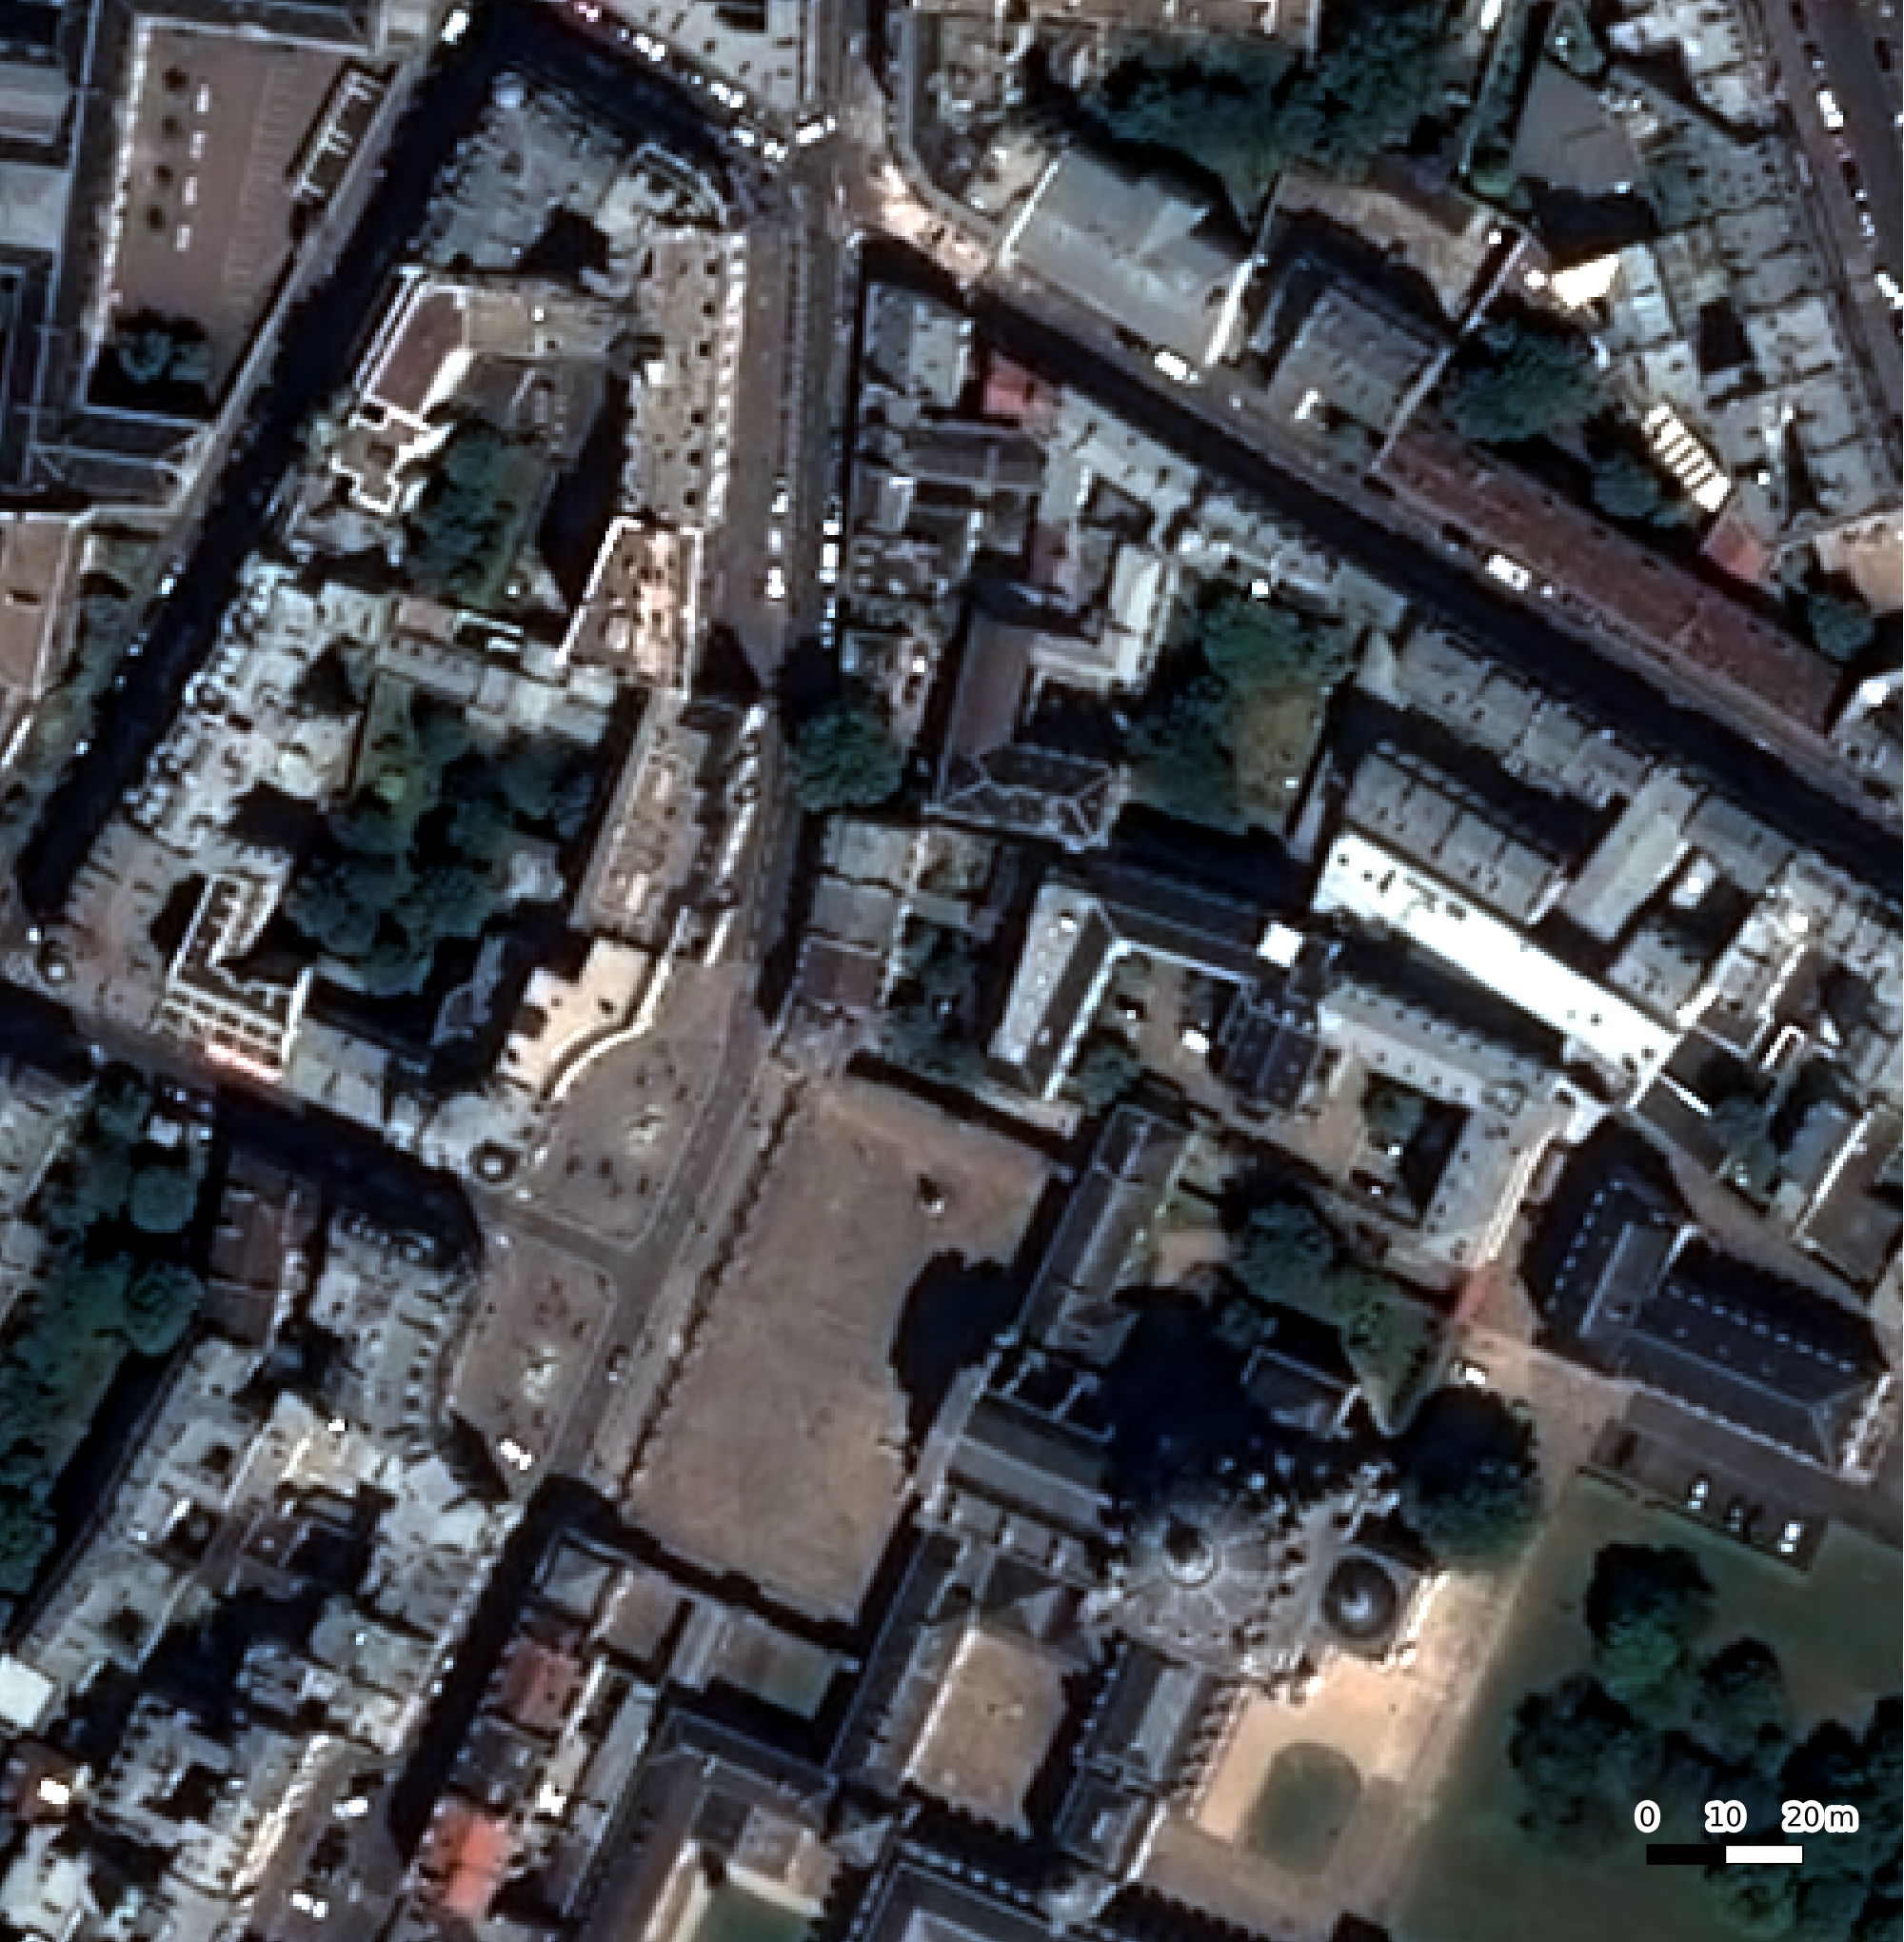
\includegraphics[height=6cm]{Images/0_Intro/Paris_Ortho.png}
        \caption{Pléiades image \copyright \acrshort{cnes} 2017, Distribution AIRBUS DS}
        \label{fig:VDG_ortho}
    \end{subfigure}\hfill
    \begin{subfigure}[t]{0.5\linewidth}
        \centering
        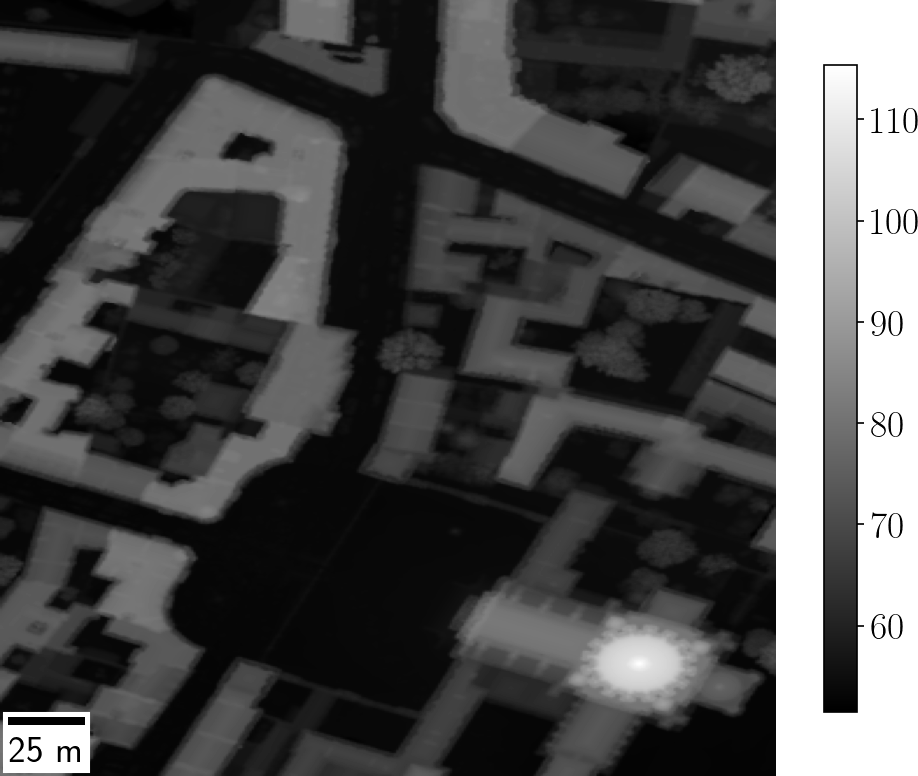
\includegraphics[height=6cm]{Images/0_Intro/Paris_DSM.png}
        \caption{Digital Surface Model from \acrshort{lidar} HD (unit: m)}
        \label{fig:VDG_dsm}
    \end{subfigure}
    \caption{Satellite image over Val-de-Grâce, Paris at $0.5$m of resolution, and a \acrshort{dsm} over the same area.}
    \label{fig:intro_dsm_example}
\end{figure}

There are multiple ways of creating a \acrshort{dsm} from airborne sensors such as planes, drones or satellites. The first way is to use \acrshort{radar} interferometry, as done by Sentinel-1 satellites \cite{geudtner_sentinel-1_2014}, the Shuttle Radar Topography Mission (SRTM) \cite{farr_shuttle_2007} or TanDEM-X (\cite{krieger_tandem-x_2007}). Typical planimetric resolutions obtained are in the range of a dozen meters (10m for TanDEM-X or 30m for the SRTM). Another method is to construct \acrshort{dsm} by means of stereophotogrammetry \cite{tao_comprehensive_2001}, \ie the science of recovering 3D information from optical images. For this method, images of a scene are acquired from different points of view. Depth information is recovered from the parallax effect between images, \ie the fact that objects closer to the sensors present a greater shift between images than objects in the background. This effect is also what allows depth perception in human vision. \Cref{fig:parallax} illustrates the parallax effect, where the top of Eiffel Tower has a greater position shift in both image than its basis. As current optical satellites have a sub-meter resolution, it is possible to massively produce \acrshort{dsm} covering the globe using photogrammetry for a relatively low cost. The altimetric resolution is typically around one meter, although it depends of the different acquisition angles of the satellites. A final method for producing \acrshort{dsm} is to use \acrfull{lidar} \cite{khosravipour_generating_2016}. Using \acrshort{lidar} allows to obtain very good accuracy. For instance, the \acrfull{ign} is using \acrshort{lidar} to cover the french territory, with a planimetric accuracy of 25 centimeters, and an altimetric resolution of 5 centimeters allowing to observe very small objects. Acquisitions campaigns such as this one are carried out using airborne vehicles, and are thus costly and take a lot of time. Therefore, photogrammetry \acrshort{dsm}s are currently the best solution to produce \acrshort{dsm}s covering the globe  with a sub-meter resolution for relatively low costs. This thesis will therefore mainly considered \acrshort{dsm}s produced using stereophotogrammetry.

\begin{figure}
    \begin{subfigure}[t]{0.32\linewidth}
        \flushleft
        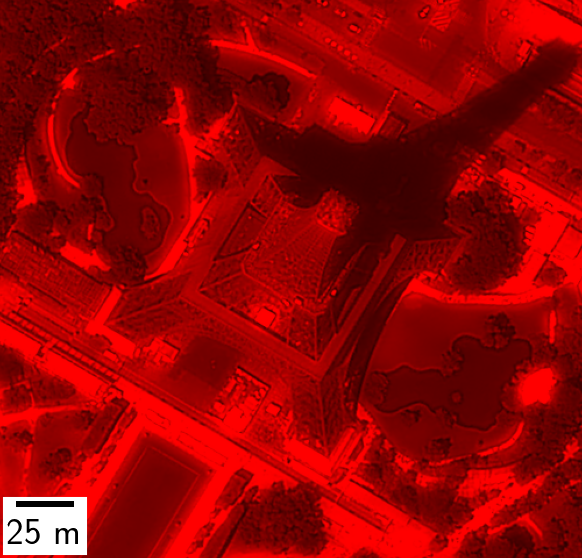
\includegraphics[width=\linewidth]{Images/0_Intro/eiffel_tower_left.png}
        \caption{Left Image (Red channel)}
        \label{fig:eiffel_tower_left}
    \end{subfigure}\hfill
    \begin{subfigure}[t]{0.32\linewidth}
        \centering
        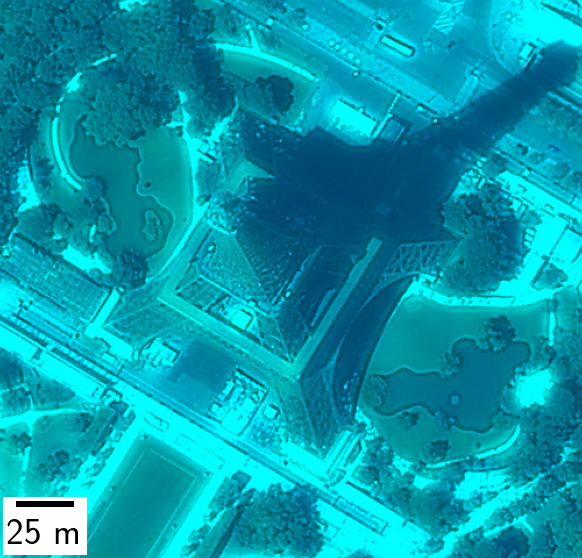
\includegraphics[width=\linewidth]{Images/0_Intro/eiffel_tower_right.png}
        \caption{Right Image (Blue and Green channel)}
        \label{fig:eiffel_tower_right}
    \end{subfigure}\hfill
    \begin{subfigure}[t]{0.32\linewidth}
        \flushright
        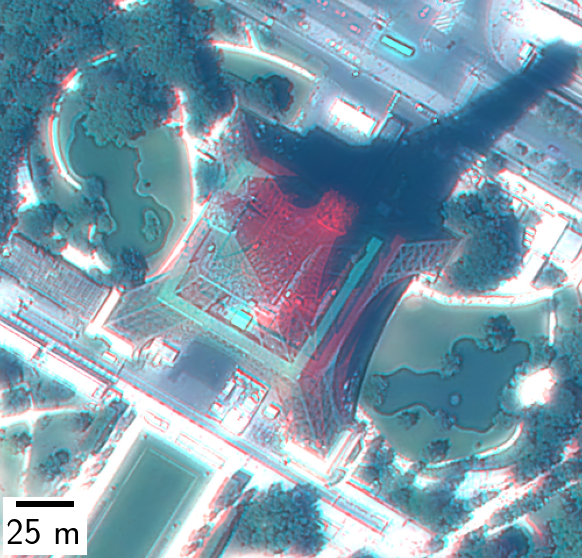
\includegraphics[width=\linewidth]{Images/0_Intro/eiffel_tower_ana.png}
        \caption{Anaglyph}
        \label{fig:eiffel_tower_ana}
    \end{subfigure}
    \caption{Example of the parallax effect: the top of the Eiffel Tower has a greater shift in-between images than its basis. The anaglyph contains the red band of the left image and the green and blue bands of the right image. (Pléiades © \acrshort{cnes} 2023, Distribution AIRBUS DS)}
    \label{fig:parallax}
\end{figure}


In this context, \acrshort{cnes} - the French Space Agency - is planning to launch 4 low-cost optical satellites with Airbus Defense and Space, in order to massively produce \acrshort{dsm} using stereophotogrammetry. This mission, named \acrshort{co3d} (for \textit{Constellation Optique 3D}, \cite{melet_co3d_2020}), was conceived jointly with \acrshort{ign} to provide high resolution \acrshort{dsm} over the globe, at a $50cm$ resolution.

For thus purpose, \acrshort{cnes} developed a pipeline dedicated to process all images provided by the \acrshort{co3d} satellites automatically and at a very large scale. This pipeline is called \acrfull{cars}, and is composed of many different image processing steps. The different steps will be detailed in the first chapter, but can be summarized as follows:
\begin{itemize}
    \item Resampling of image in a convenient geometry for matching pixels
    \item Dense matching of every pixel between stereo images
    \item Triangulation of matched pixels into 3D points
    \item Rasterization, \ie projection of the 3D points onto a regular grid, therefore yielding the final \acrshort{dsm} 
\end{itemize}
The hardest and most crucial part of this pipeline is the dense matching of pixels. It is also a famous problem in computer vision, which find applications in robotics and autonomous cars for instance \cite{geiger_vision_2013}. Alongside the \acrshort{dsm} computation, one of the requirements of the \acrshort{co3d} mission is to produce a performance map indicating the estimated quality of each cell of the \acrshort{dsm}. This motivates \acrshort{cnes} to lead research in order to estimate the uncertainty amongst the \acrshort{cars} pipeline. The main objective of this thesis is therefore to characterize and propagate the uncertainty throughout this photogrammetry pipeline. Considering the complexity of the \acrshort{cars} pipeline, as well as the time constraint resulting from the future launch of the \acrshort{co3d} satellites, we mainly focus on characterizing the uncertainty of the dense matching step. After quantifying this uncertainty, we propagate it to the end of the pipeline onto the final \acrshort{dsm}.

Characterizing and quantifying uncertainty has many benefits, although it can sometimes be computationally expensive to deal with. It indeed provides additional information for better decision making and risk management. It can also allow for a better understanding of the underlying processes at stake regarding the value of interest. In many cases, uncertainty estimation is treated as a secondary objective in applications. However, jointly estimating a value and its uncertainty can lead to new strategies to reduce the uncertainty or sometimes even improve the performances of the main applications \cite{qin_uncertainty-guided_2022,chen_learning_2023,jiang_unsupervised_2024}.

Before delving into uncertainty estimation and its propagation, we first need to specify what we mean by uncertainty. Uncertainty is a situation where a measure or value of interest is not known, or not known with precision. It is subject to change, as additional information, measures or a different acquisition protocol may reduce how uncertain a value is. It can also be subjective. For instance, someone may be uncertain about the launch date of \acrshort{co3d} satellites, while someone else working at the launch pad might have the answer. This highlights the fact that while everyone has an understanding of what uncertainty is, it encompasses very different concepts in nature. It is common to differentiate the various types of uncertainty by dividing it into two categories: stochastic uncertainty (also called random uncertainty) and epistemic uncertainty \cite{hora_aleatory_1996,frank_treatment_1999}.

Stochastic uncertainty refers to every situation of purely aleatoric nature. For instance, the result of a coin throw, random noise on a \acrshort{ccd} captor or the Brownian movement of a particle. An operator typically encounters this kind of uncertainty in a situation where they have access to many measures or observations of the same value of interest. It is usually modeled mathematically with a frequentist approach, using probability measures such as the uniform distribution, Gaussian distribution or the Student's $t$ distribution.

On the other hand, epistemic uncertainty refers to a situation where the value of interest is not known or ill-known due to a lack of knowledge. Think of the previous example with the launch date of satellites, or if someone was asked to guess Io's mass, one of the moons of Jupiter. There is no random process at stake here, and there is usually no point of acquiring multiple samples of the measure if we have a reliable and precise sensor. Once the value of interest is known, the uncertainty no longer exists. It has been proposed to model this kind of uncertainty using a Bayesian approach for probability, by opposition with the frequentist approach. Probabilities here represent a state of knowledge, or degree of belief, one has over the value of interest. It can be updated with additional knowledge, thus leading to the notion of prior and posterior probabilities. We will see during this thesis that other model can be used to characterize this uncertainty, for instance \textit{imprecise probabilities} and more specifically \textit{possibility distributions}. In satellite imagery, those models have been used to detect land changes \cite{lesniewska-choquet_specialite_2020} for instance.

During this thesis, we contributed both to the field of photogrammetry and to the field of imprecise probabilities. Here is a quick overview of the contents that can be found in the following chapters:
\begin{itemize}
    \item \Cref{chap:stereophotogrammetry} introduces the different stereophotogrammetry concepts considered in this thesis. It focuses on the stereo pipeline developed by \acrshort{cnes} and its sources of uncertainty, which will be considered in our applications.
    \item \Cref{chap:representation_of_uncertainty} will introduce the different uncertainty models considered in this thesis, mainly possibility distributions and copulas.
    \item In \Cref{chap:joining_credal_sets}, we propose different methods for creating specific multivariate uncertainty models based on the models introduced in \Cref{chap:representation_of_uncertainty}. We also study the relationships between the methods we introduced.
    \item \Cref{chap:propagating} uses the concepts of \Cref{chap:representation_of_uncertainty} and the results of \Cref{chap:joining_credal_sets} to propagate uncertainties modeled by possibility distributions in a part of the dense matching step of the stereo pipeline.
    \item \Cref{chap:epistemic_uncertainty} also uses possibility distributions, but this time to characterize the uncertainty of the dense matching step itself. Using this method, we are able to obtain confidence intervals at the end of the dense matching step. 
    \item \Cref{chap:elevation_intervals} propagates the disparity intervals to the end of the pipeline, in the form of elevation intervals on the final \acrshort{dsm}. 
\end{itemize}

As our contributions concern two distinct fields of research, multivariate uncertainty and photogrammetry, readers with a level of expertise in one field might be less interested in the second field. We tried, as much as possible, to write each chapter so it can be read and followed by everyone, although some details might need additional knowledge in a field of expertise. To help readers to navigate through chapters according to their center of interests, here is an attempt to classify each chapter into its field of research.
\begin{itemize}
    \item \Cref{chap:stereophotogrammetry} focuses on stereophotogrammetry.
    \item \Cref{chap:representation_of_uncertainty,chap:joining_credal_sets} focuses on the modelling of uncertainty, with \Cref{chap:joining_credal_sets} delving into more advanced concepts.
    \item \Cref{chap:propagating} joins both fields, but leans a bit more towards uncertainty propagation than towards photogrammetry. 
    \item \Cref{chap:epistemic_uncertainty,chap:elevation_intervals} also attempt to join both fields of research, but focuses almost completely on photogrammetry.
\end{itemize}

The rest of this section lists the contributions and research events that occurred during this thesis.
\noindent National conferences:
\begin{itemize}
    \item LFA 2022: ``Copules, probabilités inférieures et ensembles aléatoires : comment et quand les appliquer ?''  \cite{malinowski_copules_2022}
\end{itemize}
International conferences:
\begin{itemize}
    \item SMPS 2022: ``Copulas, Lower Probabilities and Random Sets: How and When to Apply Them?'' - \cite{malinowski_copulas_2022}
    \item ISIPTA 2023 (Special jury recognition Award): ``Uncertainty Propagation using Copulas in a 3D Stereo Matching Pipeline'' -  \cite{malinowski_uncertainty_2023}
    \item IGARSS 2024: ``Robust Confidence Intervals For Digital Surface Models Using Satellite Photogrammetry'' -  \cite{malinowski_robust_2024}
\end{itemize}
International journals:
\begin{itemize}
    \item International Journal of Approximate Reasoning: ``Uncertainty propagation in stereo matching using copulas'' -  \cite{malinowski_uncertainty_2024}
\end{itemize}
Not yet published pre-print:
\begin{itemize}
    \item Available on ArXiv: ``Robust Confidence Intervals in Stereo Matching using Possibility Theory'' - \cite{malinowski_robust_2024-1}
\end{itemize}
Workshops, poster sessions:
\begin{itemize}
    \item Belief 2022 conference: Poster presentation "Using Copulas with Random Sets"
    \item Workshop Imagin ``journée imprécision et incertitude en analyse et traitement d'images'': Funding of the event and communication, and oral presentation ``Uncertainty Propagation in Dense Matching''
    \item SFPT ``Pléiades Neo: de nouveaux satellites pour de nouveaux usages''. Oral presentation: ``Confidence Intervals for Digital Surface Models''
    \item GdR IASIS ``Télédétection et Climat''. Oral presentation ``Estimation d'Incertitudes dans la Création de Modèles Numériques de Surface issus d'Imagerie Spatiale''
\end{itemize}

\pagebreak
